\section{Proposed Approach}\label{sec:proposed_approach}
To address the challenges in predicting major oxide compositions from \gls{libs} data, we propose the development of advanced computational models capable of effectively handling the multifaceted challenges we describe in \ref{subsec:challenges}.
These issues complicate the accurate and robust prediction of elemental concentrations, necessitating advanced computational methodologies.

Our approach aims to enhance the prediction accuracy and robustness for major oxides in \gls{libs} data by leveraging specific combinations of machine learning models and preprocessors that are particularly effective at predicting individual oxides.
The models will use feature vectors $\mathbf{x} \in \mathbb{R}^N$ derived from the Masked Intensity Tensor $\mathbf{M}[\chi, l, \lambda]$ as input, where $N$ is the number of features.
The output will be Estimated Concentration Vectors $\mathbf{v} \in \mathbb{R}^{n_o}$.

As highlighted in Section~\ref{sec:related-work}, the literature suggests that various models and preprocessing techniques are adept at handling high-dimensional data, multi-collinearity, and matrix effects.
The literature also indicates that different machine learning models perform better on some oxides than others.
These challenges and model-specific strengths suggests that an optimal approach would involve hybrid methodology, integrating multiple models and preprocessing steps tailored to the specific characteristics of the data.
This could include leveraging ensemble learning techniques to combine the predictions of various models, implementing dimensionality reduction techniques like \gls{pca} to mitigate high-dimensionality issues, and employing robust preprocessing strategies to address multi-collinearity and matrix effects.
Furthermore, a systematic evaluation through cross-validation and hyperparameter tuning would be essential to fine-tune the models for the best performance on the specific oxides of interest.
The notion of using multiple models per oxide is supported by the advent of models such as the \gls{moc}~\cite{cleggRecalibrationMarsScience2017} model, which combines the predictions of multiple models using a predetermined weighting for each model's predictions on a per-oxide basis.
While this approach improved accuracy compared to individual models, it required manual tuning of the weights for each model.
This manual tuning presents limitations, including the analysis required to determine appropriate weights and the risk of suboptimal weighting.
Given these limitations, it is reasonable to explore techniques that can automate the weighting process while still leveraging the strengths of multiple models.
To fulfill these criteria, we chose to adopt a stacking ensemble approach.
Stacking, as described in Section~\ref{subsec:stacked-generalization}, is a method that utilizes multiple base estimators trained on the same data, whose predictions are then used to train a meta-learner.
By combining a diverse set of base models, stacking can correct for the biases of individual models.
Since each model focuses on different patterns within the data, stacking mitigates the inherent biases of individual models by estimating and correcting for these biases.
Leveraging the strengths of multiple models that each approach the problem differently can lead to better generalization on unseen data.
This is achieved by using a meta-learner to discern patterns in the base predictors' outputs\cite{wolpertstacked_1992, survey_of_ensemble_learning}, with the added benefit of automating and potentially improving upon the manual tuning employed by the \gls{moc} model.
However, it is crucial to consider the training of the base models to prevent data leakage and overfitting.
As emphasized by \citet{cvstacking}, if the base models are trained on the same dataset, the meta learner might favor certain base models over others.
This can cause the meta learner to be influenced by the same patterns and biases that the base models are susceptible to, leading to overfitting.
To mitigate this risk and ensure generalizability, a cross-validation strategy should be employed to ensure that the meta learner's training data accurately reflects the true performance of the base learners.

We adopted an experimental approach to empirically evaluate the potential of various models and preprocessing techniques for use in our stacking ensemble.
This ensured our selections were informed by the literature review while allowing for independent assessment and validation.

To systematically address the challenges in predicting major oxide compositions from \gls{libs} data, we have devised an approach that integrates model and preprocessing selection, an experimental framework, evaluation and comparison, and the construction of a stacking ensemble.

Firstly, we conducted a literature review and performed preliminary experiments to select a diverse set of machine learning models and preprocessing techniques.
These include ensemble learning models, linear and regularization models, neural network models, scaling methods, dimensionality reduction techniques, and data transformations.
This selection process is detailed in Section~\ref{sec:model_selection}.

Next, in Section~\ref{subsec:validation_testing_procedures}, we introduce our validation and testing procedures, delineate our data partitioning and cross-validation strategy, and present our evaluation and comparison metrics, all developed to ensure robust performance assessment and generalizability of the models by addressing challenges such as data leakage and uneven distribution of extreme values.

We present the metrics we use to evaluate the performance of our models in Section~\ref{subsec:evaluation_metrics}.
These metrics include the \gls{rmse} for accuracy and the sample standard deviation of prediction errors for robustness.
By evaluating both cross-validation and test set metrics, we ensure a thorough assessment of the models' generalizability and performance on unseen data.

Next, we implemented an optimization framework using Optuna as a foundation~\cite{optuna_2019}.
This framework facilitates automated hyperparameter optimization, allowing us to efficiently explore a vast search space of model and preprocessing configurations.
The specifics of this framework are discussed in Section~\ref{sec:optimization_framework}.

Finally, the top-performing configurations are used to construct a stacking ensemble.
This ensemble leverages the strengths of multiple models, with a meta-learner trained to optimize the final predictions.
The process of constructing and validating this stacking ensemble is described in Section~\ref{subsec:stacking_ensemble}.

By following this structured approach, we aim to enhance the prediction accuracy and robustness for major oxides in \gls{libs} data, ultimately leading to more reliable and generalizable models.

\subsection{Model and Preprocessing Selection}

Choosing the right models and preprocessing techniques for \gls{libs} data analysis is a challenging task. 
As the literature highlighted in Section~\ref{sec:related-work} suggests, a variety of models and preprocessing techniques promise to be adept at handling data that exhibit high-dimensionality, multi-collinearity, and matrix effects.
The literature also indicates that different machine learning models perform better on some oxides than others.
These challenges and model-specific strengths suggests that an optimal approach would involve combining multiple models. 
This notion is supported by the advent of models such as the \gls{moc}~\cite{cleggRecalibrationMarsScience2017} model, which combines the predictions of multiple models using a predetermined weighting for each model's predictions on a per-oxide basis.
While this approach improved accuracy compared to individual models, it required manual tuning of the weights for each model.
This manual tuning presents limitations, including the analysis required to determine appropriate weights and the risk of suboptimal weighting.
Given these limitations, it is reasonable to explore techniques that can automate the weighting process while still leveraging the strengths of multiple models.
To fulfill these criteria, we chose to adopt a stacking ensemble approach. 
Stacking, as described in Section~\ref{subsec:stacked-generalization}, is a method that utilizes multiple base estimators trained on the same data, whose predictions are then used to train a meta-learner.
By combining a diverse set of base models, stacking can correct for the biases of individual models.
Since each model focuses on different patterns within the data, stacking mitigates the inherent biases of individual models by estimating and correcting for these biases.
This approach of leveraging the strength of multiple models that each model the problem differently can lead to better generalization on unseen data by automating and potentially improving upon manual tuning through the use of a meta-learner to discern patterns in the base predictors' outputs. \cite{wolpertstacked_1992, survey_of_ensemble_learning}
However, some consideration has be made towards training of the base models in order to prevent data leakage and overfitting.
As emphasized by \citet{cvstacking}, if the base models are trained on the same dataset, the meta learner might favor certain base models over others.
This can cause the meta learner to be influenced by the same patterns and biases that the base models are susceptible to, leading to overfitting.
To mitigate this risk and ensure generalizability, a cross-validation strategy should be employed to ensure that the meta learner's training data accurately reflects the true performance of the base learners.

We adopted an experimental approach to empirically evaluate the potential of various models and preprocessing techniques, to be used in our stacking ensemble, ensuring that our selections were informed by our literature review while also allowing for independent assessment and validation.

We had several considerations to guide our selection of preprocessing techniques.
Firstly, our review of the literature revealed that there seems to be no consensus on a single, most effective normalization method for \gls{libs} data.
Therefore, we included traditional normalization methods in our experiments, such as z-score normalization, Min-Max scaling, and Max Absolute scaling.
This approach allowed us to determine which normalization method was most effective for our dataset. 
Additionally, dimensionality reduction techniques are considered by the literature to be effective techniques for \gls{libs} data due to its high dimensionality. 
Specifically, \gls{pca} has been widely adopted by the spectroscopic community as an established dimensionality reduction technique~\cite{pca_review_paper}. 
However, \citet{pca_review_paper} make the case that the assumptions for \gls{pca} regarding linearity of the data are only met up to a certain point, after which it breaks. 
They argue that this non-linearity inherent in the data makes \gls{kernel-pca} a valid candidate for \gls{libs} data. 
Based on their review of the field, and our own review of the literature, not many have studied the effectiveness of \gls{kernel-pca} in the context of \gls{libs} data. 
Therefore, we decided to include this in our experiments to further assess its potential. 
In addition to the non-linearity, \citet{pca_review_paper} also argue that the assumptions of normality in the data are not always met in \gls{libs} data. 
For this reason, we decided to include power transformation and quantile transformation in our experiments, as models such as \gls{pca} benefit from a normal distribution of the data. 
We assume that models such as \gls{pls} may also benefit from a more Gaussian-like data distribution, given that the model is partly based on \gls{pca}.

While these preprocessing techniques are not an exhaustive list, they represent a diverse set of methods.
Techniques such as feature selection were not considered in this study to limit its scope and due to time constraints.

We also had several requirements for the model selection.
The selected models for experimentation had to be diverse to ensure sufficient breadth in our results, enabling informed decisions about which models to include in the final stacking ensemble pipeline.
Additionally, the models had to be suitable for regression tasks. 
In the absence of research specific to \gls{libs} data, we selected models that have shown promise in other domains.
Our literature review found that a variety of models fit this criteria.
For example, \citet{andersonPostlandingMajorElement2022} demonstrated that models such as \gls{gbr}, \gls{pls}, \gls{lasso}, and \gls{rf} were each effective at predicting different major oxides from \gls{libs} data. 
Additionally, \citet{svrforlibs} showed that \gls{svr} outperforms \gls{plsr} in predicting \ce{Si}, \ce{Ca}, \ce{Mg}, \ce{Fe}, and \ce{Al} using \gls{libs} data.
As a result, we included \gls{gbr}, \gls{pls}, \gls{lasso}, \gls{rf}, and \gls{svr} in our experiments.

In the neural network domain, \cite{ann_libs_soil_analysis} showed that on \gls{libs} data their 3-layer \gls{ann} relative error of prediction for \ce{Ca}, \ce{Fe}, \ce{Al} was below 20\%.
Likewise, \citet{yangConvolutionalNeuralNetwork2022} showed that \gls{cnn} outperformed methods such as \gls{logreg}, \gls{svm} and linear discriminant analysis at correctly classifying twelve different types of rocks based on \gls{libs} data. 
While this example for \gls{cnn} is a classification task, \gls{cnn} can be adjusted for regression tasks by changing the loss function and output layer.
Based on these factors, we decided to include \gls{ann} and \gls{cnn} in our experiments to further increase the diversity of our model selection.

To further bolster our selection pool, we chose to include models that were in the same family of models as those that showed promise in the literature.

\gls{xgboost} was included as an option based on its promising accuracy in various settings.
For example \citet{xgboost_in_biomedicie} showed that \gls{xgboost} outperformed models such as \gls{rf} and \gls{svm} in predicting biological activity based on quantitative description of the compound's molecular structure. 
Another example is \citet{xgboost_in_heart_disease} that used \gls{xgboost} to predict heart disease, where \gls{xgboost} outperformed \gls{rf} and \gls{etr} at correctly classifying patients with heart disease.
Due to these factors and the limited study of \gls{xgboost} in the context of \gls{libs} data, we decided to include it in our experiments.

Following the same logic, we included \gls{ngboost}. 
\gls{ngboost} is a recent model introduced by \citet{duan_ngboost_2020} that, according to their work, improves upon \gls{gbr} by using a more sophisticated loss function and a more advanced gradient boosting algorithm.
Limited research has been conducted using this algorithm in the context of \gls{libs} data. 
However, \citet{ngboost_landslide} showed that \gls{ngboost} outperformed \gls{xgboost} and \gls{rf} in correctly determining landslide-prone fields, with an AUC of 0.898 compared to 0.871 and 0.863 for \gls{xgboost} and \gls{rf}, respectively.

Finally, \gls{ridge}, \gls{enet}, \gls{etr}, and \gls{lasso} were included in various studies and showed promising results, even if they were not the top performers in their respective studies.
Therefore, we chose to include these in our experiments to further diversify our model selection. 

Table~\ref{tab:preprocessing-models} summarizes the preprocessing techniques and models selected for our experimentation.

\begin{table}[ht]
\centering
\begin{tabularx}{\columnwidth}{>{\raggedright\arraybackslash}X}
\toprule
\textbf{Normalization / Scaling:} \\
\midrule
Z-Score Normalization \\
Min-Max Normalization \\
Max Absolute Scaling \\
Robust Scaling \\
Norm 3 \\
\midrule
\textbf{Transformation Methods:} \\
\midrule
Power Transformation \\
Quantile Transformation \\
\midrule
\textbf{Dimensionality Reduction Methods:} \\
\midrule
PCA \\
Kernel PCA \\
\midrule
\textbf{Model Types:} \\
\midrule
\textbf{Regression Models:} \\
\quad Partial Least Squares \\
\quad Support Vector Regression \\
\quad Elastic Nets \\
\quad Least Absolute Shrinkage and Selection Operator \\
\quad Ridge Regression \\
\textbf{Ensemble Models:} \\
\quad Random Forest \\
\quad Gradient Boost Regression \\
\quad Extra Trees Regression \\
\quad XGBoost \\
\quad Natural Gradient Boosting \\
\textbf{Neural Networks:} \\
\quad Artificial Neural Networks \\
\quad Convolutional Neural Networks \\\bottomrule
\end{tabularx}
\caption{Overview of Preprocessing Techniques and Models}
\label{tab:preprocessing-models}
\end{table}
\subsection{Validation and Testing Procedures for Model Evaluation}\label{subsec:validation_testing_procedures}
This section describes the validation and testing procedures our experiments follow.
Selecting appropriate testing procedures is crucial for ensuring the validity and reliability of the results.
For that reason, we delineate a methodological approach that ensures our models are accurate and generalizable.

We have chosen to test and evaluate all our experiments using both cross-validation and a separate test set.
Evaluating results solely on the test set could lead to models that are overly specialized to the test set.
This occurs when searching for the optimal configuration of hyperparameters specifically tailored to the test set.
However, our objective is to develop models that demonstrate high accuracy and robustness, even on entirely unseen data.
To achieve this, we employ k-fold cross-validation to ensure our models have high generalizability, thereby increasing the likelihood that they will perform as expected on new data.

We use an $80\%/20\%$ split for training and testing sets. The training set is further subdivided into $4$ folds, which are used for cross validation.

While we employ conventional techniques like holdout sets and k-fold cross validation, the dataset we use imposes additional challenges to the process.

One of the primary challenges is preventing data leakage.
As per concentration matrix $\mathbf{C}$ in Section~\ref{sec:problem_definition}, each target only has one ground truth concentration value per oxide.
However, each target is shot at multiple locations, resulting in multiple instances of the same target in the dataset, as shown in Table~\ref{tab:final_dataset_example}.
Although the intensity values vary for each location, they fundamentally represent measurements of the same target.
If we were to randomly split the dataset, some locations from a target could end up in the testing set while others remain in the training set.
This would cause data leakage, as the testing set would no longer consist solely of unseen targets.
To prevent this, we ensure that each target is represented only once in the dataset by grouping data from all locations on a given target.

Furthermore, the limited availability of data, as mentioned in Section~\ref{sec:problem_definition}, poses another significant challenge due to the difficult collection process.
The dataset we use consists of 408 samples, which is relatively large by \gls{libs} standards.
However, there are only a few samples with concentration values for the oxides in the targets that are either very high or very low compared to the rest of the data, which we call extreme values.
These less frequent high and low concentration values can be problematic.
If such values end up in the test set, the model may be evaluated on data points outside the range it was trained on.
This situation can lead to an inaccurate assessment of the model's performance, as it might not handle these less common concentration ranges effectively.

When performing a random split of the dataset into multiple folds for cross-validation, as well as for training and testing sets, this small number of extreme values can result in an uneven distribution.
The presence or absence of these extreme values in any given fold can heavily influence the model's performance metrics.
If extreme values are disproportionately allocated to the testing set, the resulting model may struggle to generalize accurately.
This uneven distribution can lead to models that perform well on the majority of the data but fail to predict accurately for these extreme concentration values, which are critical in many practical applications.
Conversely, if the scarce extreme values are disproportionately assigned to the training set, the model may become overly specialized in handling these extreme values, potentially leading to overfitting.
This means the model might perform well on the training set, including the extreme values, but fail to generalize effectively to new, unseen data, especially if the test set does not contain similar extreme values.
This could result in an inaccurate assessment of the model's performance, as the test set would not adequately challenge the model's ability to predict across the full range of data variability.

\begin{figure*}[h!]
    \centering
    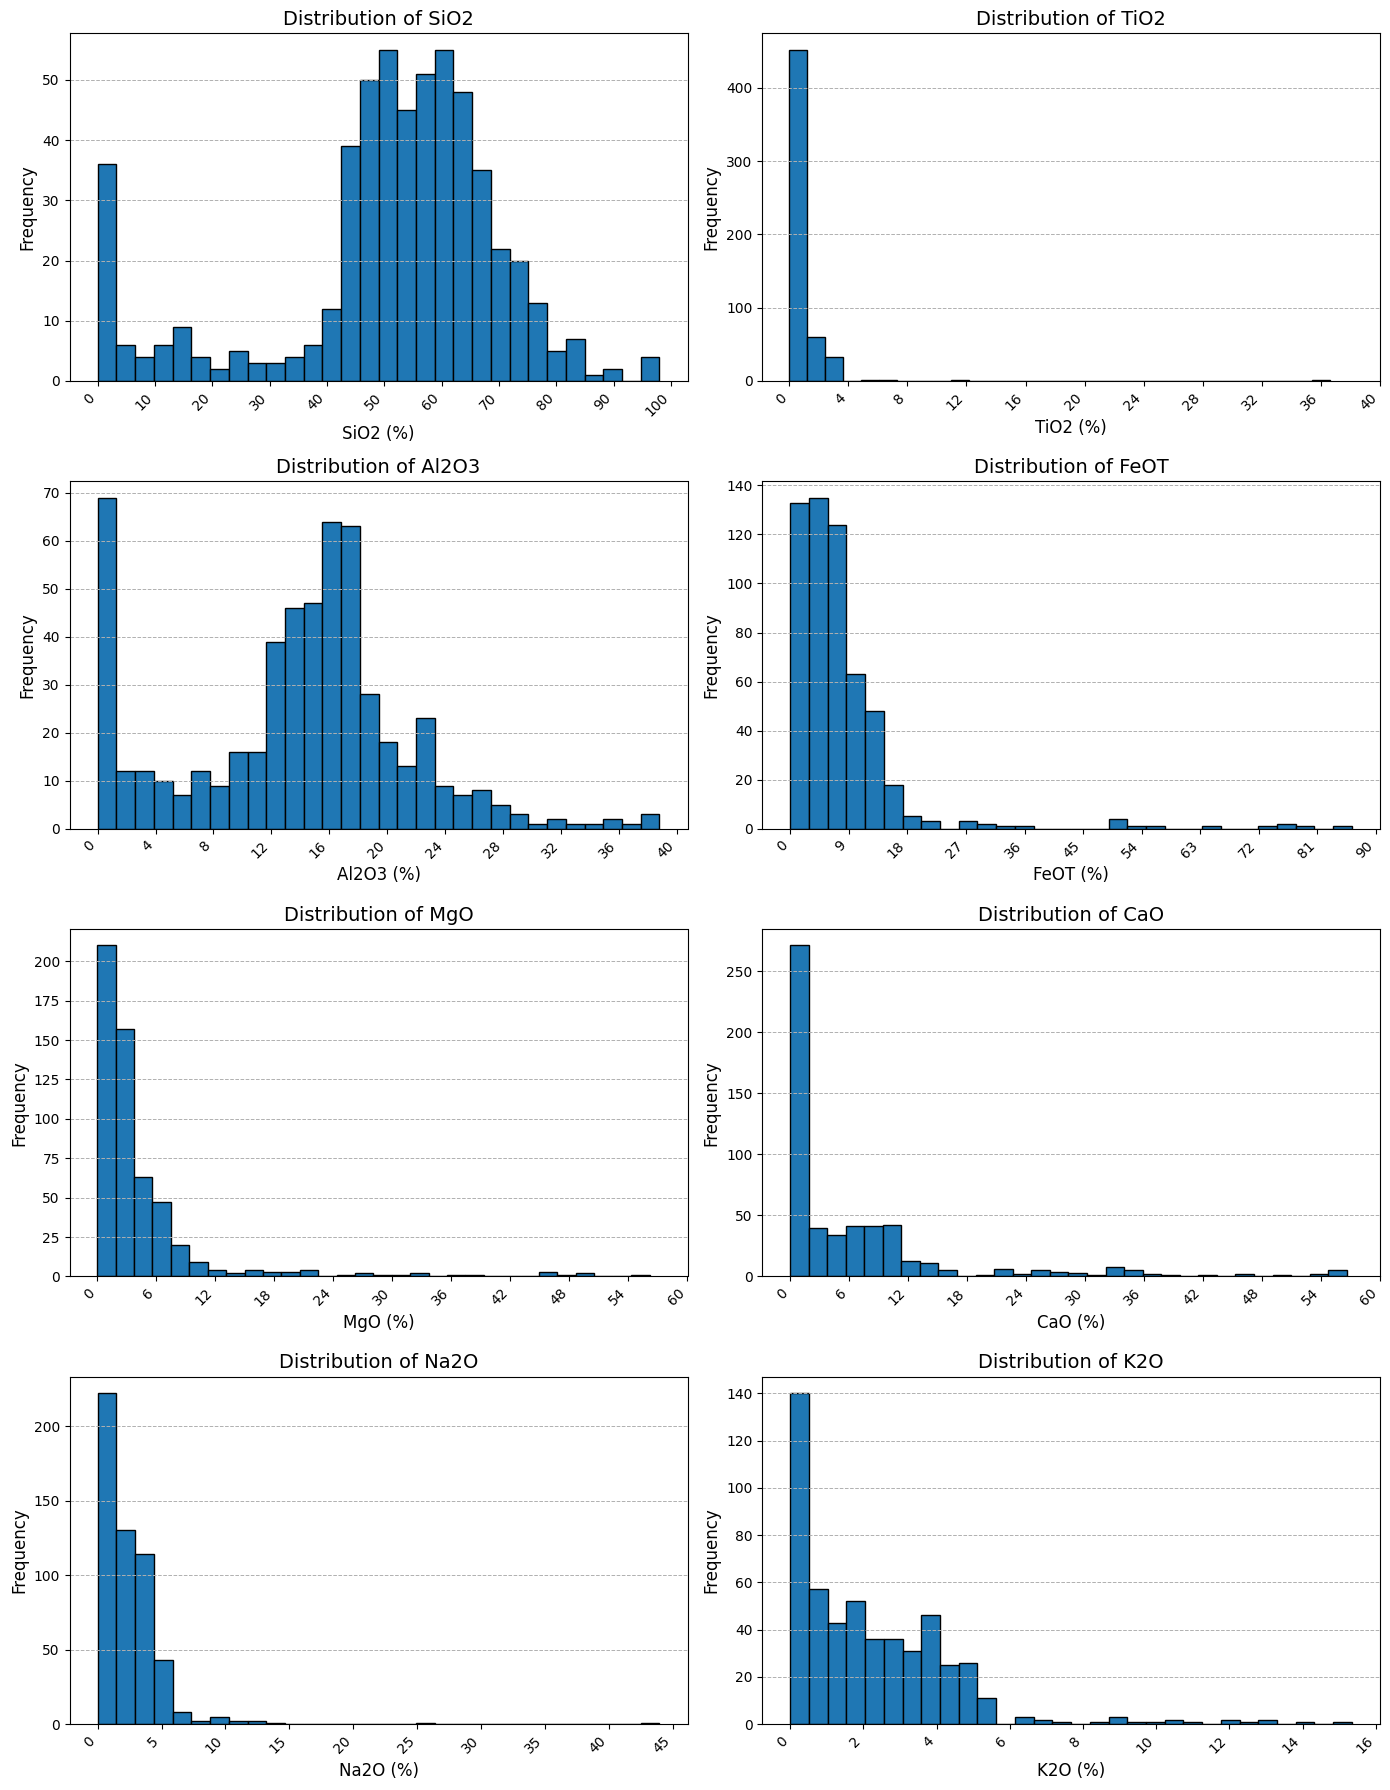
\includegraphics[width=\textwidth]{images/oxide_distributions.png}
    \caption{Distributions of various oxide concentrations in the dataset. The histograms show the frequency of concentration values for \ce{SiO2}, \ce{TiO2}, \ce{Al2O3}, \ce{FeO_T}, \ce{MgO}, \ce{CaO}, \ce{Na2O}, and \ce{K2O}.}
    \label{fig:oxide_distributions}
\end{figure*}

Figure~\ref{fig:oxide_distributions} illustrates the distributions of various oxide concentrations in our dataset.
Across all oxides, there is a general pattern of skewed distributions, with concentrations heavily weighted towards lower values.
This is particularly notable in \ce{TiO2}, \ce{FeO_T}, \ce{MgO}, \ce{CaO}, and \ce{Na2O}.
\ce{SiO2} and \ce{Al2O3} show more variability, with \ce{SiO2} exhibiting a bimodal distribution.
These distributions confirm the presence of extreme values across all oxides, which are significantly overrepresented or underrepresented, further complicating the model training process.

This necessitates careful dataset partitioning to ensure that the model training process accounts for these challenges, improving the generalizability and robustness of the models.

\subsubsection{Dataset Partitioning}\label{subsubsec:dataset_partitioning}
To ensure rigorous evaluation of our models and to address the challenges of data leakage and uneven distribution of extreme values, we have implemented a customized k-fold data partitioning procedure. 
This approach divides the dataset into $k$ folds, which it uses to define cross-validation data sets, as well as a training set and a test set.
The procedure ensures that all data points from a given target are only present in one of the $k$ folds, overcoming the challenge of data leakage we mention above.
Additionally, it ensures that extreme values are handled by redistributing them evenly across the training folds, preventing any single fold from being disproportionately influenced by these values.

\begin{algorithm}
\caption{Data Partitioning With Extreme Value Handling}
\label{alg:custom_kfold_cv}
\begin{algorithmic}[1]
\Require Dataset $\mathbf{D}$, group column $g$, target column $t$, number of splits $k$, percentile $p$, random seed $\textit{seed}$
\Ensure Training and validation sets for cross-validation $\mathbf{T}_\text{cv}$, training set $\mathbf{D}_\text{train}$, and test set $\mathbf{D}_\text{test}$
\State \label{line:seed} Set random seed for reproducibility if $\text{seed}$ is not None
\State \label{line:remove_duplicates} Remove duplicate entries based on $g$ and sort by $t$
\State \label{line:assign_folds} Assign fold numbers sequentially from 0 to $k-1$ to unique targets
\If{extreme values handling is enabled}
    \State \label{line:identify_extremes} Identify extreme values at percentiles $p$ and $1-p$
    \State \label{line:reassign_extremes} Reassign extreme values to folds $0$ to $k-2$
\EndIf
\State \label{line:merge_folds} Merge fold assignments information into the original dataset
\State \label{line:split_dataset} Split dataset into test set $\mathbf{D}_\text{test}$ (fold $k-1$) and remaining data $\mathbf{D}_\text{train}$
\State \label{line:create_folds} Create $k-1$ training and validation sets
\For{each fold $i$ from 0 to $k-2$}
    \State $\mathbf{T}_\text{train}[i] \gets \mathbf{D}_\text{train} \setminus \text{fold}_i$
    \State $\mathbf{T}_\text{val}[i] \gets \text{fold}_i$
    \State Append $(\mathbf{T}_\text{train}[i], \mathbf{T}_\text{val}[i])$ to $\mathbf{T}_\text{cv}$
\EndFor
\State \label{line:remove_fold_column} Remove fold column from all datasets
\State \Return $\mathbf{T}_\text{cv}, \mathbf{D}_\text{train}, \mathbf{D}_\text{test}$
\end{algorithmic}
\end{algorithm}

The procedure outlined in Algorithm~\ref{alg:custom_kfold_cv} begins by setting a random seed for reproducibility if one is provided (Line~\ref{line:seed}).
This ensures that the results are consistent across different runs of the algorithm.
Next, the dataset is processed to remove any duplicate entries based on the group column $g$ and then sorted by the target column $t$ (Line~\ref{line:remove_duplicates}).
This step ensures that each group is uniquely identified and ordered appropriately.
The dataset we illustrate in Table~\ref{tab:final_dataset_example} would require a group column $g$ of "\texttt{Target}" to group the data by target.
The target column $t$ refers to the column with the target variable, which would be the oxide for which we are predicting the concentration, for example, \ce{SiO_2}.
By sorting the dataset by the target column $t$, we ensure that the data is ordered by the target concentration values in ascending order.

Fold numbers are then assigned sequentially using a modulo operation to ensure a random-like distribution of the unique targets across the folds (Line~\ref{line:assign_folds}).
This means that, while the assignment process follows a sequence, the resulting distribution of targets is effectively randomized.
Fold numbers start in 0 and go up to $k-1$, as implied by the modulo operation.
If handling of extreme values is enabled, the algorithm identifies the top and bottom percentiles of the target values (Line~\ref{line:identify_extremes}).
These extreme values are then reassigned to the training folds (0 to \( k-2 \)), ensuring they are evenly distributed across these folds (Line~\ref{line:reassign_extremes}).

The fold assignments are then merged into the original dataset, as described in Line~\ref{line:merge_folds}.
Essentially, this step enables the partitioning steps that follow, by ensuring each data item has an associated fold number.
Following this, the dataset is divided into a test set, which always consists of the data points assigned to fold $k-1$, and the remaining data forms the training set, as outlined in Line~\ref{line:split_dataset}.
The training data is further divided into $k-1$ sets for cross-validation. 
For each fold $i$ where $i \in \{0, 1, \ldots, k-2\}$, we create a cross-validation training set $\mathbf{T}_\text{train}[i]$ by excluding the $i$-th fold from the set of $k-1$ folds, and use the $i$-th fold as the validation set $\mathbf{T}_\text{val}[i]$.
These pairs of training and validation sets are then appended to the list of cross-validation sets $\mathbf{T}_\text{cv}$ (Line~\ref{line:create_folds}).

Finally, the fold indicator column is removed from all datasets before returning the final partitions (Line~\ref{line:remove_fold_column}).
The fold indicator column was added to keep track of which data points belong to which folds, which is crucial for ensuring that data points are correctly partitioned into their respective training and test sets during cross-validation. 
This cleanup step ensures that the fold information does not interfere with subsequent data processing or model training.

The final output of this procedure consists of:
\begin{itemize}
    \item A set of tuples \(\mathbf{T}_\text{cv}\), where each tuple contains a training set and a validation set.
    \item The overall training set \(\mathbf{D}_\text{train}\), consisting of all the data points not in the test set.
    \item The test set \(\mathbf{D}_\text{test}\), distinct from the training set.
\end{itemize}

The data partitioning does not modify the original dataset; it merely partitions it.
For that reason, each of the datasets that are returned has the same structure as shown in Table~\ref{tab:final_dataset_example}.

Our method for handling extreme values ensures that the test set does not include samples outside the range seen in the training set.
This approach addresses several critical challenges and represents a deliberate trade-off to improve the reliability of our model evaluation:

Firstly, it mitigates the risk of uneven distribution of extreme values, which can disproportionately affect model performance metrics.
If extreme values are unevenly distributed between the training and test sets, the evaluation of the model can be heavily skewed, leading to unreliable and misleading performance metrics.
By redistributing extreme values evenly across the training folds, we ensure a more balanced and fair assessment of the model's capabilities during cross-validation.

Secondly, this trade-off allows for a more stable and reliable assessment of the model's performance on typical data points.
While the test set may be less representative of the full range of data, particularly regarding rare extreme values, the evaluation focuses on the model's ability to generalize from the training data to new data within the same distribution range.
This is prudent because, in many practical applications, the reliability of the model on typical data points is more critical than its performance on rare extremes.
By using cross-validation in conjunction with a separate test set, we ensure that the model is robust and performs well under typical conditions.

However, it is important to recognize the limitation this approach introduces: excluding extreme values from the test set means we can only confidently assess the model's performance within the range of the test set.
If we receive predictions outside this range, we cannot reliably assert their accuracy, as the model has not been fully evaluated on such data.
This could potentially make the model less useful in scenarios where predictions on extreme values are critical.
Nevertheless, cross-validation partially mitigates this issue by allowing the model to learn from extreme values during the training and validation phases, thereby improving its robustness.
Metrics obtained from cross-validation provide a broader picture of the model's accuracy and robustness across the entire dataset, including extreme values.

Therefore, although our approach may make the test set less representative of the full dataset, it is a deliberate trade-off aimed at achieving a more accurate and reliable evaluation of the model's generalization performance.

Our method is inspired by the approach described by \citet{andersonImprovedAccuracyQuantitative2017}.
They employed a similar strategy to assess the performance of their PLS model, using k-fold cross-validation and a separate test set.
Their process involved dividing the full set of laboratory data into five folds, using four for cross-validation and combining them as the final training set, while the fifth fold served as a test set.
For consistency, we also use $k = 5$ for our data partitioning.
Given that the $k$-th fold is used as the test set, having $k=5$ results in 4 folds for cross-validation.

Additionally, by using $k = 5$ folds, we have effectively chosen an 80\%/20\% split between the training and testing datasets.
In our experience, this ratio maximizes the training set's capacity for effective model learning while ensuring that the testing set is sufficiently representative to provide an accurate assessment of the model's performance on new data.
Allocating too much data to the testing set could compromise the comprehensiveness of the training set, undermining the model's ability to generalize effectively due to the limited availability of data.

\subsubsection{Cross-Validation}
% Section on cross validation approach
\subsection{Optimization Framework}\label{sec:optimization-framework}




















In this section we introduce our optimization framework built on the Optuna framework.
Optuna is a hyperparameter optimization framework designed for direct integration with Python. Its dynamic embedding capability allows hyperparameters to be defined and adjusted within the code during execution, providing additional flexibility and ease of debugging. 
Optuna uses advanced sampling strategies to explore promising areas of the search space and employs pruning techniques to terminate unpromising trials early, optimizing computational resource use. 
It also supports scaling across multiple machines by distributing the optimization process, allowing for concurrent optimization. 
Additionally, tools are provided to identify and focus on the most impactful parameters, aiding in the efficient handling of high-dimensional search spaces. \cite{optuna_2019} 
Because an essential aspect of our study is to identify the optimal configuration of model and preprocessing techniques for that model on a per-oxide basis, these factors make Optuna an ideal choice as the basis of our optimization framework.
Optunas flexibility meant that it was easy to customize the optimization process to solve this problem and integrate it with our existing codebase.

At the core of the framework is what is referred to as the objective function.
The objective function acts as the primary building block, where the sampling parameters are set for the preprocessing techniques and the models and is the function that is minimized. % rephrase
Sampling parameters in this context relate to the range of values or options that the optimizer can choose from.

Because we want to identify not only the best model configuration, but also the best preprocessing configuration for that model, we have combined the sampling of the model and preprocessing parameters into a single objective function.
By doing this, we can optimize the entire pipeline in a single step, rather than optimizing the model and preprocessing steps separately.
% We 
With such a setup, Optuna will attempt to optimize any permutation of scaler, transformer, dimensionality reduction, and model hyperparameters throughout the optimization process.
This allows us to fully utilize Optunas sampling and pruning strategies, minimizing wasted time and computational resources on poor configurations.

\begin{algorithm}
\caption{Hyperparameter Optimization Framework}
\label{alg:hyperparameter_optimization_framework}
\begin{algorithmic}[1]
\Require Dataset $D$, Model $m$, Number of Trials $N$, Random Seed $seed$, Sampler \texttt{sampler}, Pruner \texttt{pruner}
\Ensure Trial data, including metrics and configuration for each trial

\State \textbf{Initialize:} Set random seed for reproducibility if seed is not None \label{step:initialize}
\For{each trial $t$ from 1 to $N$} \label{step:trial_loop}
    \Statex // Sample hyperparameters for $m$ using \texttt{sampler} and \newline \hspace*{1.2em} instantiate it 
    \State $m'$ $\gets$ \texttt{sample\_hyperparameters()} \label{step:sample_hyperparameters}
    \Statex
    \Statex // Sample and instantiate preprocessors using \texttt{sampler}
    \State \text{scaler} $\gets$ \texttt{sample\_scaler()}
    \State \text{transformer} $\gets$ \texttt{sample\_transformer()} \textbf{or} \text{NONE}
    \State \text{dim\_reduction} $\gets$ \texttt{sample\_dim\_reduction()} \textbf{or} \text{NONE}
    \Statex
    \Statex // Construct pipeline of preprocessors in that order
    \State \text{pipeline} $\gets$ [\text{scaler}, \text{transformer}, \text{dim\_reduction}]
    \Statex
    \Statex // Apply data partitioning
    \State $T_{cv}, D_{train}, D_{test} \gets \text{apply data partitioning to } D$
    \Statex
    \Statex // Apply preprocessing to $D_{train}$ and $T_{cv}$
    \State $D_{train}'$ $\gets$ \texttt{pipeline\_apply}($D_{train}$, \text{pipeline})
    \State $T_{cv}'$ $\gets$ \texttt{pipeline\_apply}($T_{cv}$, \text{pipeline})
    \Statex
    \State $CV_{metrics}$ $\gets$ \texttt{cross\_validate}($m'$, $T_{cv}'$, \text{pipeline}) 
    % \State $T_{cv}' \gets \text{pipeline\_apply}(T_{cv}, \text{pipeline})$
    % % \State $D_{train}' \gets \text{apply preprocessing to } D_{train}$
    % \State $T_{cv}' \gets \text{apply preprocessing to } T_{cv}$
    % \Statex
\EndFor
\State Save the best configuration, hyperparameters, and performance metrics \label{step:save_best_configuration}
% Might want to remove below and instead return all configurations
\State \Return the best configuration across all models and preprocessors \label{step:return_best_configuration}

\end{algorithmic}
\end{algorithm}% This increases the likelyhood at identifying the 

% create names for evaluation metrics
% 



% Optuna for its flexibility and efficiency in exploring the vast search space of configurations.
% Optuna allows for great flexiblity in exploring various search spaces due to its modular design.
% In addition to this modularity, Optuna uses a "define-by-run" optimization strategy.
% Rather than being confined to a fixed order and range of exploration, Optuna can dynamically adjust regions based on the results of previous trials.
% Introduction of the optimization framework
    % What is the goal of the optimization framework?
    % Why Optuna?
        % Explanation of what optuna is and why it is useful for our purposes
        % Should elaborate on this:
            % This framework facilitates automated hyperparameter optimization, allowing us to  efficiently explore a vast search space of model and preprocessing configurations.
% how did we do it?
    % Maybe talk about how we designed it in this way
    % pros cons ** maybe
    % Considerations at the very least
    % Talk about how the objective function was constructed, the order of things, considerations with this, the fact that we are trying to minimize and what metrics we are minimizing
    % 
% show diagram or pseudocode
% Explain why we did it this way
    % Why did we choose this approach?
    % What are the benefits of this approach?
    % How does this approach help us achieve our goal?

   
    
% Next, we implemented an experimental framework using the Optuna optimization library~\cite{optuna_2019}.
% This framework facilitates automated hyperparameter optimization, allowing us to efficiently explore a vast search space of model and preprocessing configurations.
% The specifics of this framework are discussed in Section~\ref{sec:optimization_framework}.


% Optuna uses python syntax instead of some propriety syntax
% Optuna brings the optimization into the space of the program rather than outside
    % Meaning you can embed it directly in functions etc.
    % Easier to debug
    % Can use python language such as looping etc.
% Instead of having parameters set you change them so they are sampled using the suggest_* methods
    % This is also helpful because it allows you to optimize any parameter, even for preprocessing etc. in the same objective function
% There are two parts of the hyperparameters optimizer: Sampling strategy and Pruning strategy
    % Sampling strategy determines where to look
        % Uses bayesian filtering to find places where it has had the best results and focus in on those
        % As Optuna tries to minimize/maximize the objective function it focuses in on the best areas and makes more trials there
        % There are multiple samplers - Even the traditional ones
        % Choosing the right sampler is sort of a heuristic 
    % Pruning strategy can terminate trials early that are not promising so that the compute can be dedicated to more promising trials
        % Basically trials that have a slow start and will never be able to make up for that slow start, are pruned
% Optuna is very easy to scale up. It allows you to use a single database across multiple machines
    % This means that Optuna will let you use multiple computers to optimize over the search space at the same time
    % Its called asynchronous parallelization of trials - One trial could start later than the other
    % Near linear scaling with the number of machines
% Has tools to help you determine most important parameters to avoid curse of dimensionality
    % get_param_importances
    % It works by running a small number of trials and then returns this information to you
    % Helps you dial in where optuna should be focusing to get most optimal results

